El algoritmo de steepest-descent hace uso del gradiente de la función a optimizar para buscar la dirección de máximo descenso que es tangente al punto dado. Entonces el algoritmo optimiza en dicha dirección de descenso usando un algoritmo auxiliar de optimización lineal. A parte del criterio de parada estándar también se usa el criterio $|| - \bigtriangledown f(x_k) || < \epsilon $

\begin{wrapfigure}{r}{0.5\textwidth}
\vspace{-4.8em}%
\hfill%
\hspace{-6ex}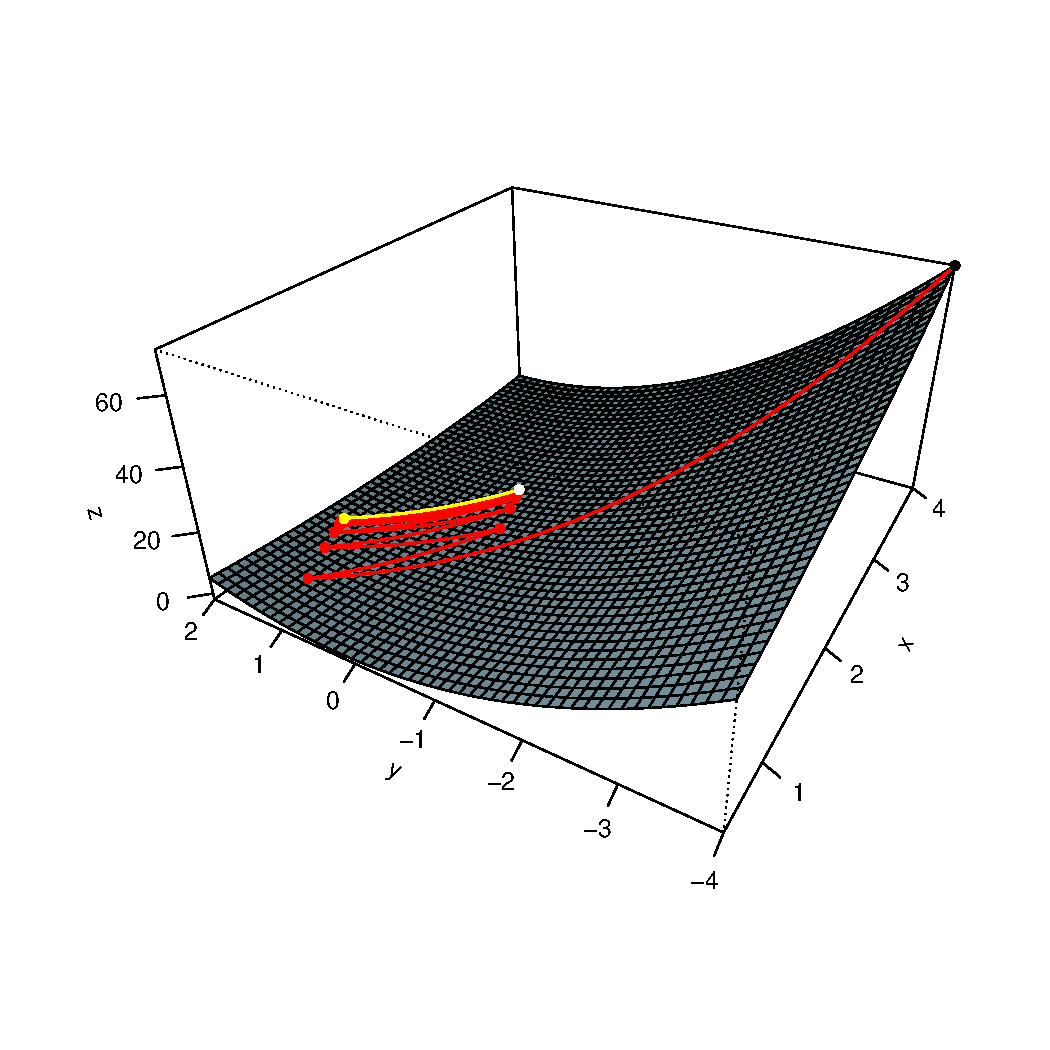
\includegraphics[width=0.9\linewidth]{../graphs/gregory_fun/steep/steep.pdf}%
\hfill\hbox{}
\vspace{-3.5em}
\caption{\small gregory-karney en $x_0=(4,-4)$ del \hyperref[tab:steep]{cuadro \ref*{tab:steep}}} \label{fig:steep1}
\vspace{-3em}
\end{wrapfigure}

Para implementarlo usamos el algoritmo de la sección áurea para optimizar en las rectas, con el mismo criterio que en el algoritmo de \hyperref[sub:alg-rose]{rosenbrock}. Este algoritmo en general da buenos resultados, aproximándose a mínimos locales de forma efectiva. 

Uno de los problemas que tenemos con nuestra implementación es el ``underflow'' y ``overflow'' cuando tiende el resultado a 0 o a infinito. Concretamente los NaN de la tabla inferior se deben a que al evaluar el punto final en la función resulta en un valor que excede la capacidad del tipo básico de la máquina, resultando en un valor infinito en uno de los pasos intermedios de la evaluación de la función.

Aquí un cuadro con los resultados de algunas de las pruebas que hemos realizado:

\begin{table}[H]
\hfill\begin{tabular}{|c|cccccc|c|}\hline
\bf point   & \bf path & \bf eval & \bf grad & \bf diff        & \bf final                         & \bf value ($\approx$) & \bf function                    \\\hline\hline
(0.001,10)  & 1001     & 67002    & 1001     & 10.2313         & (8.97279e-71,-1.40843)            & -2.4e-06              & \multirow{3}{*}{patata}         \\
(10,10)     & 503      & 33636    & 503      & -nan            & (4.87463e+154,443.202)            & -nan                  &                                 \\
(10,0)      & 76       & 5027     & 76       & -nan            & $\approx$(1.34e+156,0)            & -nan                  &                                 \\\hline\hline
(4,4)       & 1001     & 67002    & 1001     & 8.00037         & $\approx$(1.54,1.74)              & -0.0004               & \multirow{7}{*}{gregory-karney} \\
(-4,-4)     & 1001     & 67002    & 1001     & 23.9994         & (2.45958,0.25639)                 & 0.0006                &                                 \\
(4,-4)      & 1001     & 67002    & 1001     & 72.0007         & (2.45942,0.256639)                & -0.0007               &                                 \\
(0,0,0)     & 1001     & 67002    & 1001     & $\approx$0.0007 & $\approx$(2.68,2.71,0.43)         & -0.0007               &                                 \\
(3,3,3)     & 1001     & 67002    & 1001     & 2.99967         & $\approx$(3.32,1.29,1.57)         & 0.0003                &                                 \\
(0,0,0,0,0) & 1001     & 67002    & 1001     & $\approx$0.003  & $\approx$(4.8,4.53,2.3,2.63,0.62) & -0.003                &                                 \\
(5,5,5,5,5) & 1001     & 67002    & 1001     & 14.9957         & $\approx$(5.2,3.47,3.7,1.36,1.3)  & 0.004                 &                                 \\\hline
\end{tabular}\hfill\hbox{}
\caption{Resultados del algoritmo de steepest-descent con $\epsilon=0.0005$} \label{tab:steep}
\end{table}
\vspace{-1em}

\begin{wrapfigure}{l}{0.5\textwidth}
\vspace{-5.3em}%
\hfill%
\hspace{-6ex}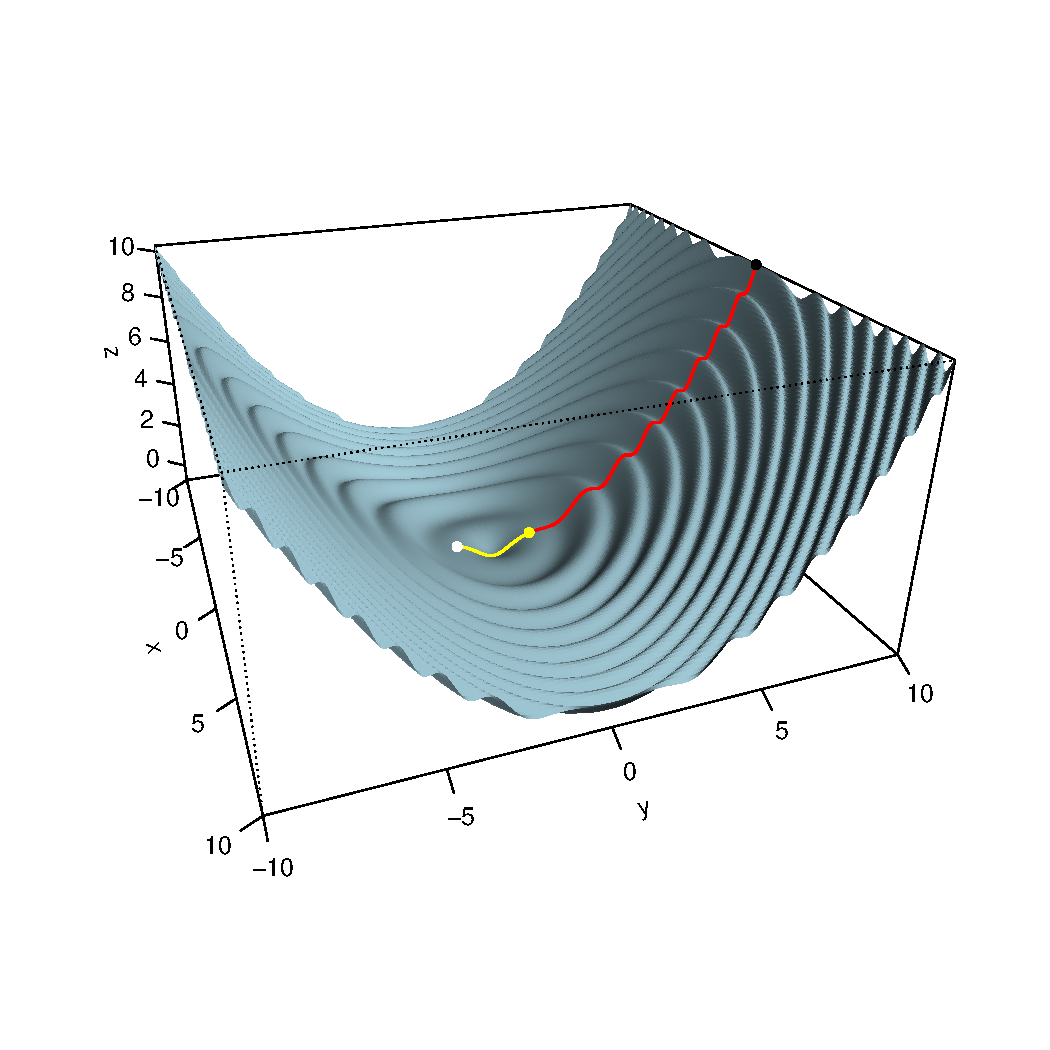
\includegraphics[width=0.9\linewidth]{../graphs/patata_func/steep/steep.pdf}
\hfill\hbox{}
\vspace{-3.5em}
\caption{\small f. patata en $x_0=(0.001,10)$ del \hyperref[tab:steep]{cuadro \ref*{tab:steep}}} \label{fig:steep2}
\vspace{-4.5em}
\end{wrapfigure}


Hay que señalar que al igual que con el algoritmo de \hyperref[sub:alg-rosen]{rosenbrock}, se pueden producir ciclos que hagan que a partir de cierto punto no se mejore más la solución conseguida.

Un caso de esto es la figura del latera, que muestra comoel algoritmo comienza a saltar entre puntos con pendiente muy plana, hasta llegar al máximo de iteraciones programado. Esta figura es ilustrativa ya que si se compara con la \hyperref[fig:rosen1]{figura \ref*{fig:rosen1}} del algoritmo de rosenbrock, steepest-descent es capaz de encontrar la dirección correcta en la que optimizar.